\chapter{On Multimedia Analysis and Retrieval}
\epiquote{All our knowledge begins with the senses, proceeds then to the understanding, and ends with reason.}{Immanuel Kant}
\label{chapter:theory_multimedia_analysis_and_retrieval}

This chapter introduces the most important fundamentals regarding multimedia data, the analysis of multimedia data and the use of derivatives in information retrieval and processing systems. The main sources used in this chapter are the books \emph{Multimedia Retrieval} by H. Blanken et al \cite{Blanken:2007multimedia} and \emph{Similarity Search -- The Metric Space Approach} by P. Zezula et al. \cite{Zezula:2006similarity}, which both provide excellent introductions into the respective fields.

%\epiquote{Quote}{Author}
%%%%%%%%%%%%%%%%%%%%%%%%%%%%%%%%%%%%%%%%%%%%%%%%%%%%%%%%%%%%%%%%%%%%%%%%%%%%%%%%%%%%%

\section{Multimedia Data and Multimedia Collections}
\label{section:multmedia_data}

Multimedia data is ubiquitous and used in different forms in every area of our daily lives, be it private or professional. With the broad adoption of the smartphone in the early 2000s, virtually every person on this planet now literally holds the tools required not only to consume but also produce multimedia information in the form of text, images, videos and audio snippets. Fueled by this technological progress, the past few decades have seen a staggering development in both \emph{volume} and \emph{variety} of multimedia data found in the wild, e.g., on the Internet or in personal or professional data collections. 

The term \emph{multimedia} refers to a combination of one or many different \emph{media types}, such as but not limited to, aural or visual information. We distinguish between these types, based on the representation we use when working and interacting with them. Sound, for example, is formed by airpressure waves that are registered by our ears. In contrast, visual information, involves electormagnetic waves captured by our eyes. In both cases, the brain plays an important role in interpreting the underlying processes and forming the human association for the phenomenon. Similarily, we require different techniques when converting these media types from their analogue to their digital representation. We can roughly classify different media types based on their relationship with time. \emph{Static} media types (e.g., an image) do not exhibit a temporal development, wheras the information of \emph{dynamic} media types (e.g., an audio signal) depends on the time point that is being examined. \cite{Blanken:2007multimedia}

Traditionally, we often think of media information that somehow can be perceived directly by our human senses. However, media data in a wider sense may also include less apparent examples such as 3D models, motion capture data or data streams stemming from sensors or medical devices. 

Even though different media types exhibit very different characteristics in their original representation, we find some commonalities that are crucial for defining the problem of processing and analysing such data in information processing systems in general and analytics systems in particular.

\begin{description}
    \item[Analogue Correspondence] Most media types somehow reflect an analogue proces taking place in the real-world. Converting such an analogue process to the digital world often requires several steps and different representations, both in the digital and analogue world (see Examples \ref{example:representation_visual_information} and \ref{example:representation_audio_information} for images and audio respectively).

    \item[Unstructured Data] The raw, digital representation of any media type is typically highly unstructured as opposed to, for example, an entry in a database. Consequently, we do not have natural units of information that can be leveraged directly for analysis. As consequence, we often rely on derivatives of the original data when peforming analysis and data processing.
    
    \item[Semantic Gap] The different, derived representations of the original data usually highlight specific aspects thereof. Conversion between such representations is often accompanied by a loss of information, a problem often referred to as the \emph{semantic gap} \cite{Blanken:2007multimedia, Rossetto:2018thesis}.

    \item[Perceptive and Interpretative Gap] Reasoning about the content of any type of media, be it based on the original data or some derivative therof, require several steps that involve preception and interpretation of the information by a human consumer. These processes are highly subjective and my lead to different results for different people, adding to the semantic gap \cite{Rossetto:2018thesis}.
\end{description}

\begin{example}[label=example:representation_visual_information]{Digital Representation of Visual Information}{}
    \begin{wrapfigure}{L}{0.45\textwidth}
        \includegraphics[width=0.45\textwidth]{figures/example-visual-signal.eps}
    \end{wrapfigure}
    The visual information in a flat image is stored as a two dimensional array of \emph{pixels}. Each pixel consists of its color values, usually one per color channel. For example, with the RGB color model, every pixel holds three values, one for the red, green and blue channel. The number of pixels per dimension determines the \emph{resolution} of the image. Typically, we use a fixed number of bits per colour, the \emph{color depth}, which determines the number colors that can be distinguished.

    If we take, for example, a coloured image of $1000 \times 1000$ pixel, we must encode \num{3e6} individual colour values. Using \SI{8}{\bit} per colour, we end up storing \SI{24e6}{\bit}, which amounts to \SI{3}{\mega\byte} worth of uncompressed image data. Images coming from modern cameras, exhibit resolutions much higher than that.
\end{example}

\begin{example}[label=example:representation_audio_information]{Digital Representation of Aural Information}{}
    \begin{wrapfigure}{R}{0.45\textwidth}
        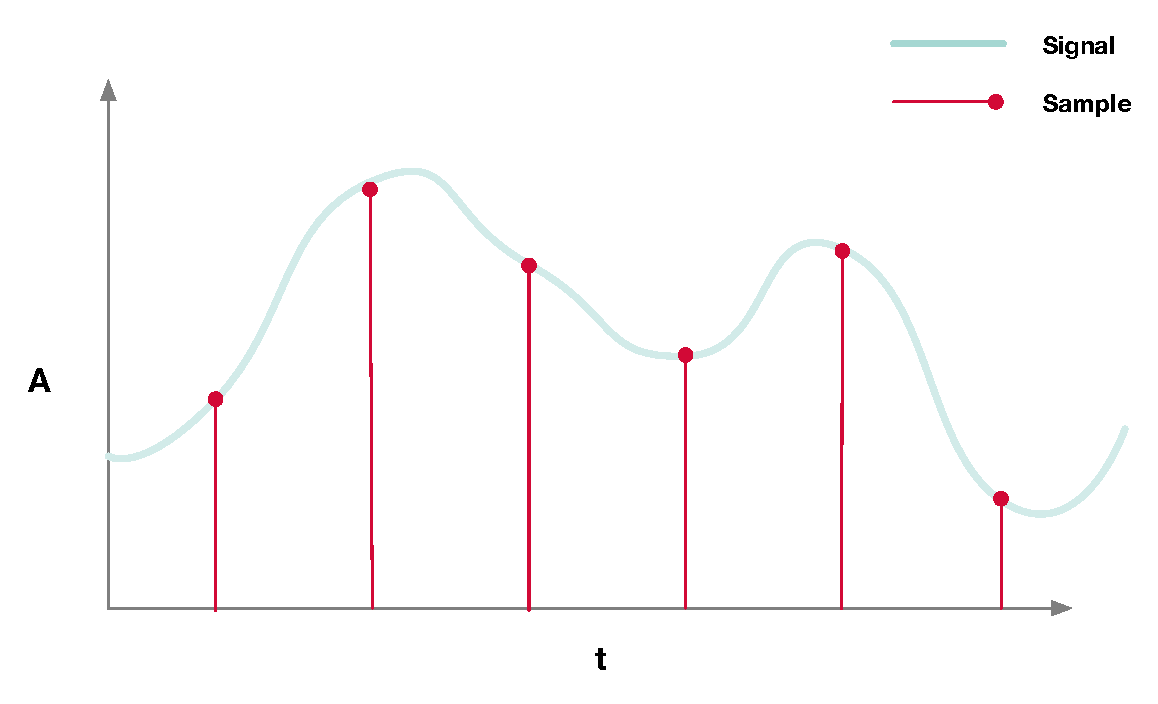
\includegraphics[width=0.45\textwidth]{figures/example-audio-signal.eps}
    \end{wrapfigure}
    The amplitude of a recorded audio signal is \emph{sampled} at a fixed rate. Each sample point consist of a value that quantizes the amplitude's energy at a given point in time to a number on a given range. An audio stream is then a sequence of these power values. The quality of the process is determined by the \emph{sample rate}, i.e., the number of samples per time unit, and the \emph{bit depth}, which determines quantization of the amplitude power.

    If we take a \SI{1}{\second} audio snippet, sampled at \SI{44}{\kilo\hertz}, we end up storing \num{44000} sample points. Using a bit depth of \SI{16}{bit} per sample, this amounts to \SI{704000}{bit} or \SI{88}{\kilo\byte} of uncompressed audio data. In modern audio systems, we typically record multiple audio channels independently, leading to even more data.
\end{example}

\begin{example}[label=example:artist_vs_image]{Structured vs. unstructured information}{}
    Let us take, for example, an entry about an artist in a database. Irrespective of the data model, there is typically a notion of an \emph{entity} (i.e., the artist) and attributes that describe the entity (e.g., hist \emph{firstname} or \emph{lastname}). This structure, expressed in the data model and the data, can be exploited to facilitate operations. If we now turn to a file containing the painting produced by the same artist, we find a series of values that encode the raw colour information for every pixel in the painting. While this information can be used to visually reconstruct the painting, it does not -- by the face of it -- give any information about the paining or its content.
\end{example}


\subsection{Metadata}

\subsection{Feature Representations}


\section{Multimedia Retrieval}

The research of domain of \emph{multimedia retrieval} deals with algorithms, methods and systems that allow for searching and obtaining items of interest from large multimedia collections. Many different subdomains for the different types of media have emerged over the years, including but not limited to image retrieval, \acrfull{mir} \cite{Simonetta:2019Multimodal}, video retrieval or 3D model retrieval.

\subsection{Similarity Search and the Vector Space Model}

In multimedia retrieval, there are two important assumptions for similiarity search. These assumptions can be summarized as follows:

\begin{itemize}
    \item For every object $c_{i}$ in a (multimedia) collection $\mathcal{C}$, there exists a feature transformation $\phi \colon \mathcal{C} \to \mathcal{F}$, that maps the object $o_{i} \in \mathcal{C}$ to a feature space $\mathcal{F}$.
    \item The feature space $\mathcal{F}$ and a to be defined distance function $\delta \colon \mathcal{F} \times \mathcal{F} \to \mathbb{R}_{\geq 0}$, constitute a metric space $(\mathcal{F},\delta)$, thus satisfying the non-negativity, identity of indiscernibles, symmetry and subadditivity condition.
\end{itemize}

The output of $\delta$ -- i.e., the calculated distance $d$ -- acts as a proxy for (dis-)similiarty between two objects $o_{i}$, $o_{j} \in \mathcal{C}$ given the feature transformation $\phi$. Hence, the closer two objects $o_{i}$, $o_{j}$ appear under the transformation, the more (dis-)similar they are. For the sake of completeness, it must be pointed out, that whether similarity is directly or inversely proportional to the distance is a matter of definition and depends on the concrete application. Also, in practice, multiple feature transformations $\phi_m$ may exist for a given media collection, leading to different feature spaces $\mathcal{F}_m$ for a collection $\mathcal{C}$ that must be considered jointly. Both aspects are usually addressed by additional \emph{correspondence} and \emph{scoring} functions.

\todo[inline]{Correspondence and score functions, score fusion}

\subsection{Approximate Nearest Neighbor Search}
The nearest neighbor search problem 

\todo[inline]{Describe techniques for approximate nearest neighbor search (ANN). Focus on a more conceptual overview of the types of algorithms rather than just enumerating concrete examples; this can be used as a build-up for discussing properties of different index structures later. }


\subsection{Beyond Similarity Search}
\todo[inline]{Retrieval and analytics techniques that go beyond simple similarity search (e.g. SOM, summarization, clustering)}

\section{Online Multimedia Analysis}
\todo[inline]{Introducing an online analysis pipeline (e.g., Pythia / Delphi).}

\section{Multimedia Analytics}
\todo[inline]{Describe how the combination of analysis }

\subsection{Beyond Similarity Search}

